\documentclass[10pt]{article}
\usepackage[margin=1in]{geometry} 
\usepackage{enumerate, xfrac, color, graphicx}
\usepackage{amsmath,amsthm,amssymb,amsfonts,mathabx}
\usepackage{booktabs}
\usepackage{caption}
\usepackage{algorithm}
\usepackage{algpseudocode}
\usepackage{pifont}
\usepackage{listings, courier}
\graphicspath{{/Users/mfzhao/Dropbox/}}
\newcommand{\N}{\mathbb{N}}
\newcommand{\Z}{\mathbb{Z}}
\lstset{breaklines=true, basicstyle=\small\ttfamily, language=R, backgroundcolor=\color{highlight}, stepnumber=5}

\definecolor{highlight}{RGB}{248,248,248}

\begin{document}
	\title{6.867 Problem Set 3}
	\maketitle
	
\subsubsection*{Neural Networks}

In some cases, we might want to use a neural network rather than another algorithm, such as SVM or logistic regression, in order to be somewhat more agnostic about the parametric form of the data-generating process. In this case, we investigate the use of neural networks, first on some toy training data sets, and subsequently on a subset of the popular MNIST dataset.

Let us first briefly review the way that neural network works. A neural network consists of a variable number of ``hidden layers``. A weight matrix maps each of your data points to a value for each node in the hidden layer. We then evaluate some ``activation function`` on each node value (typically a sigmoid function or tanh function) to get a new set of ``inputs`` for the next layer of the neural network. We continue this process until we finally arrive at our output predictions.  A schematic sketch of a neural net can be found below.

\begin{figure}[ht]
	\centering
	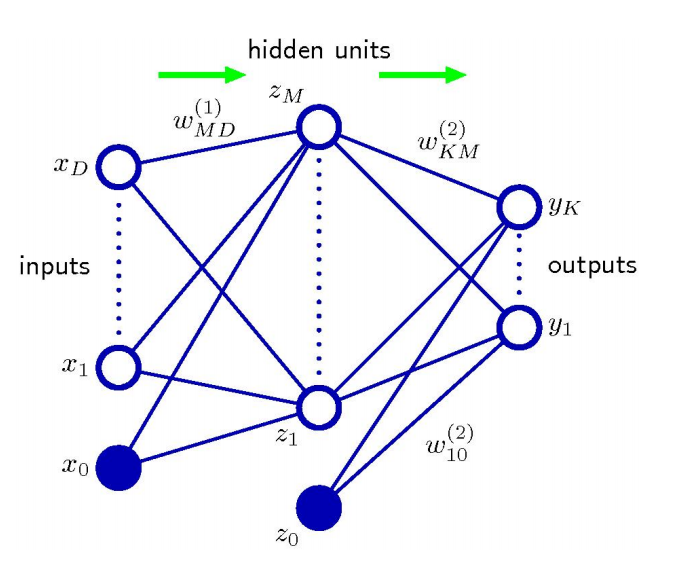
\includegraphics[height=3in]{neuralnetdiagram.png}
	\caption*{Figure 1: A schematic diagram of a neural network (taken from the homework assignment document)}
\end{figure}

Alternatively, a neural network may be specified as follows:

\begin{equation}
a_{n}^{(1)} = \sum_d w_{dn}^{(1)}x_d
\end{equation}

\begin{equation}
z_{n}^{(1)} = \sigma_1(a_n^{(1)})
\end{equation}

\begin{equation}
a_{k}^{(2)} = \sum_k w_{nk}^{(2)}z_n
\end{equation}

\begin{equation}
z_{k}^{(2)} = \sigma_2(a_k^{(2)})
\end{equation}

The most trivial neural network has only one output layer with one node, and no hidden layers. This would correspond to vanilla logistic regression. 

For the purposes of this paper, we will try to solve simple multi-class prediction problems using a neural network with one hidden layer. In order to determine the weight matrices that give us the best predictive accuracy, we will specify a loss function and perform (batch or stochastic) gradient descent. We specify our objective function as the regularized negative log-likelihood function:

\begin{equation}
J(w) = l(w) +\lambda(||w^{(1)}||^2_F + ||w^{(2)}||^2_F
\end{equation}

\noindent where $l(w)$ is

\begin{equation}
l(w) = \sum_{i=1}^N \sum_{k=1}^{K} [-y_k^{(i)}\log(h_k(x^{(i)},w)) - (1-y_k^{(i)})\log(1-(h_k(x^{(i)},w))].
\end{equation}

In order to calculate the gradient as a function of $w_1$ and $w_2$, we use the two gradient calculation expressions below:

\begin{equation}
\frac{\partial J(w)}{\partial w_{kj}^{(2)}} = -\left ( \sum_{i=1}^N z_j \left(y_k^{(i)}(1-\sigma(a_k^{(2)}) + (1-y_k^{(i)})(\sigma(a_k^{(2)})\right) \right ) + 2 \lambda w_{kj}^{(2)}
\end{equation}

\noindent and 

\begin{equation}
\frac{\partial J(w)}{\partial w_{jd}^{(1)}} = -\left ( \sum_{i=1}^N x_i \sum_{k=1}^{K} \left(y_k^{(i)}(1-\sigma(a_k^{(2)}) + (1-y_k^{(i)})(\sigma(a_k^{(2)})\right) w_{kj}^{(2)} \left(\frac{1}{1+e^{-a_{jd}^{(1)}}}\right)\left(1-\frac{1}{1+e^{-a_{jd}^{(1)}}}\right)\right ) + 2 \lambda w_{jd}^{(1)}.
\end{equation}
	
\end{document}